\chapter{Wp�yw zak��cenia sinusoidalnego na prac� algorytmu DMC}
W tym zadaniu wykorzystujemy algorytm DMC z zadania 5. Zak��cenie ma posta� sinusoidy danej wzorem:
\begin{equation}
Z(k) = Amplitude * sin(2\pi* freq / (0.5 * k) )
\end{equation}
gdzie k to numer pr�bki. 
Z(k) oznacza wektor zawieraj�cy przebieg sygna�u zak��caj�cego.
\newpage

\begin{center}
\begin{figure}[H]
\makebox[\textwidth]{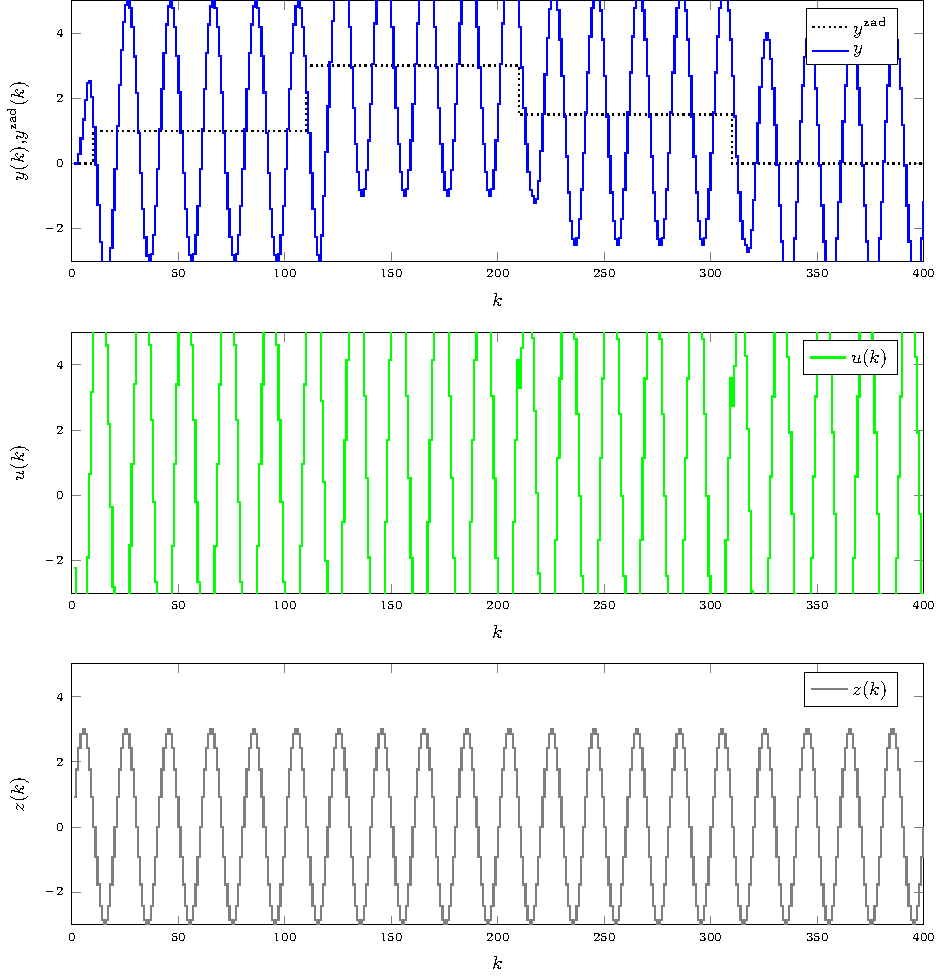
\includegraphics[width=\paperwidth]{data/exercise_6/Desired_output_plot_iter_01_ampl_3_freq_0.1_Dz_20_error_3205.4653.pdf}}
\caption{amplitude=3, freq=0.1, Dz=20, error=3205.4653}
\label{Desired_output_plot_iter_01_ampl_3_freq_0.1_Dz_20_error_3205.4653}
\end{figure}
\end{center}
\begin{center}
\begin{figure}[H]
\makebox[\textwidth]{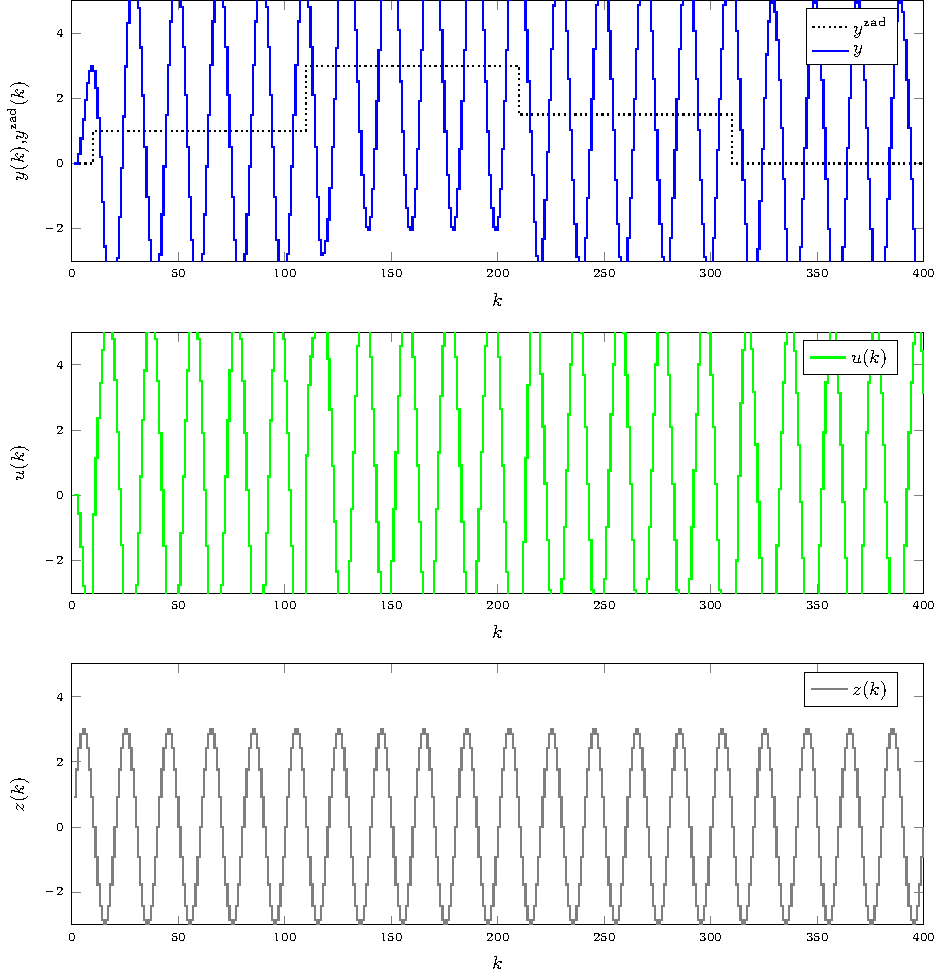
\includegraphics[width=\paperwidth]{data/exercise_6/Desired_output_plot_iter_02_ampl_3_freq_0.1_Dz_0_error_5112.5582.pdf}}
\caption{amplitude=3, freq=0.1, Dz=0, error=5112.5582}
\label{Desired_output_plot_iter_02_ampl_3_freq_0.1_Dz_0_error_5112.5582}
\end{figure}
\end{center}
\begin{center}
\begin{figure}[H]
\makebox[\textwidth]{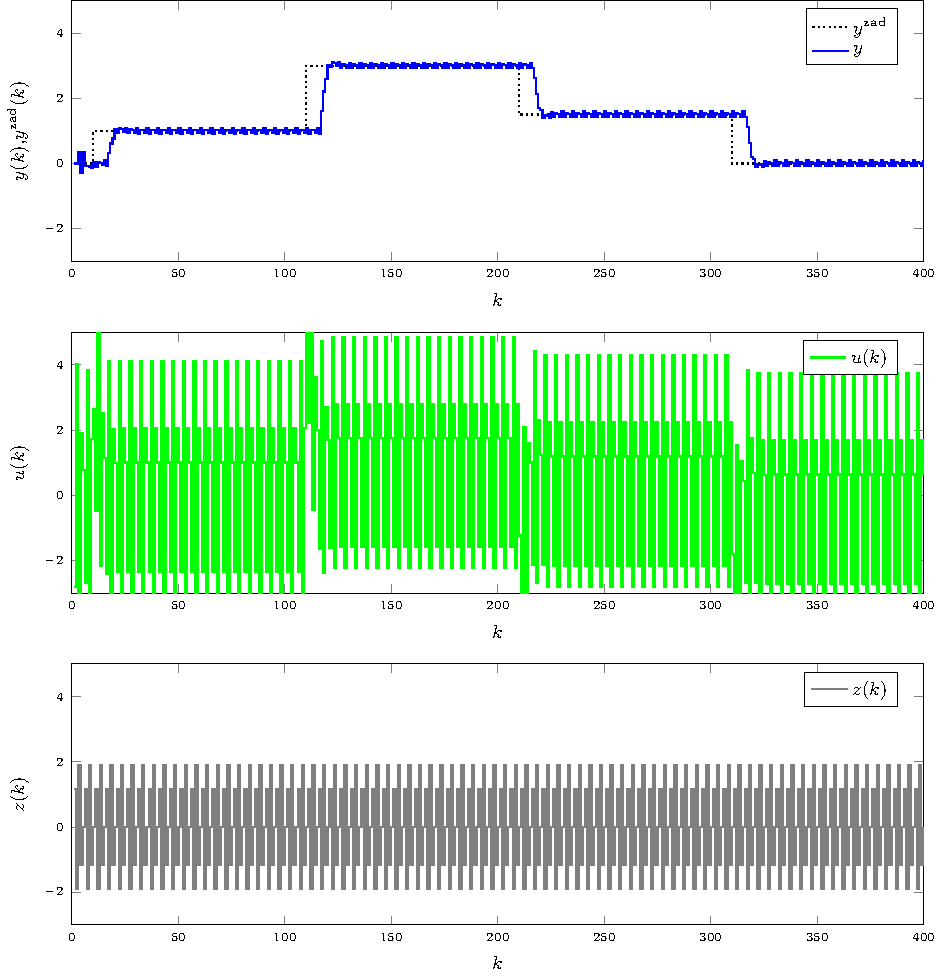
\includegraphics[width=\paperwidth]{data/exercise_6/Desired_output_plot_iter_03_ampl_2_freq_0.8_Dz_20_error_75.3829.pdf}}
\caption{amplitude=2, freq=0.8, Dz=20, error=75.3829}
\label{Desired_output_plot_iter_03_ampl_2_freq_0.8_Dz_20_error_75.3829}
\end{figure}
\end{center}
\begin{center}
\begin{figure}[H]
\makebox[\textwidth]{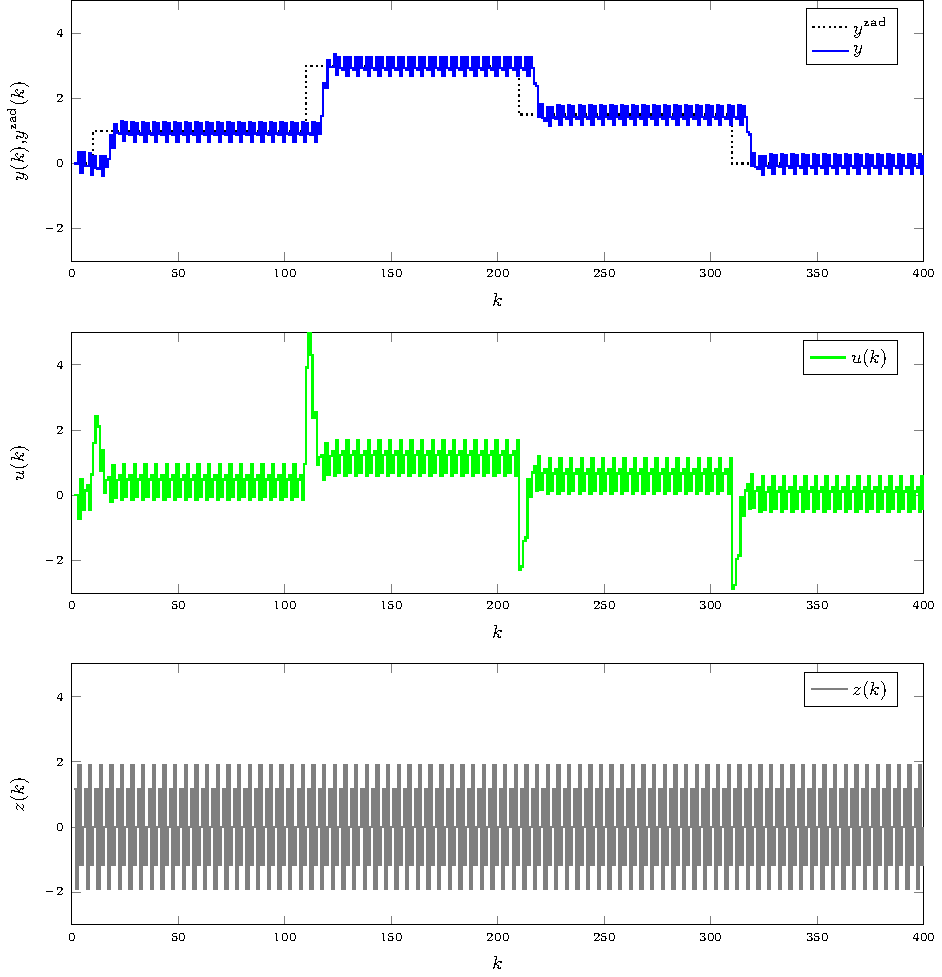
\includegraphics[width=\paperwidth]{data/exercise_6/Desired_output_plot_iter_04_ampl_2_freq_0.8_Dz_0_error_95.3365.pdf}}
\caption{amplitude=2, freq=0.8, Dz=0, error=95.3365}
\label{Desired_output_plot_iter_04_ampl_2_freq_0.8_Dz_0_error_95.3365}
\end{figure}
\end{center}
\begin{center}
\begin{figure}[H]
\makebox[\textwidth]{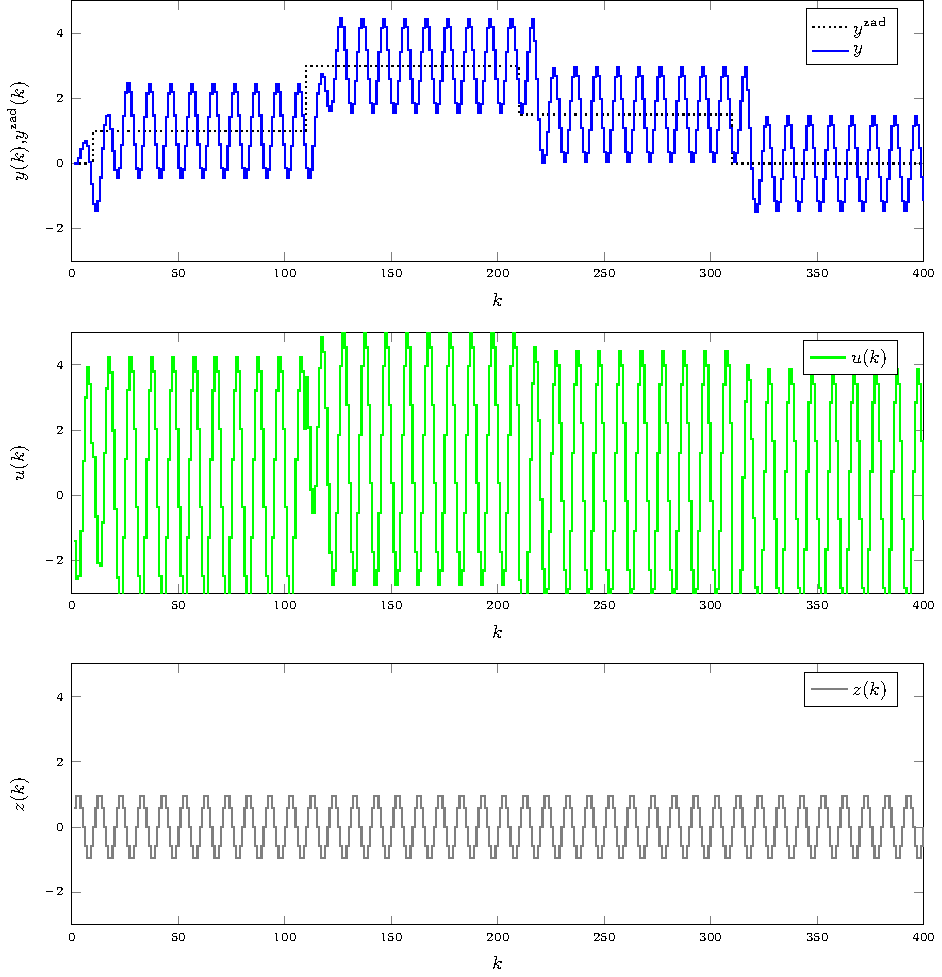
\includegraphics[width=\paperwidth]{data/exercise_6/Desired_output_plot_iter_05_ampl_1_freq_0.2_Dz_20_error_481.7742.pdf}}
\caption{amplitude=1, freq=0.2, Dz=20, error=481.7742}
\label{Desired_output_plot_iter_05_ampl_1_freq_0.2_Dz_20_error_481.7742}
\end{figure}
\end{center}
\begin{center}
\begin{figure}[H]
\makebox[\textwidth]{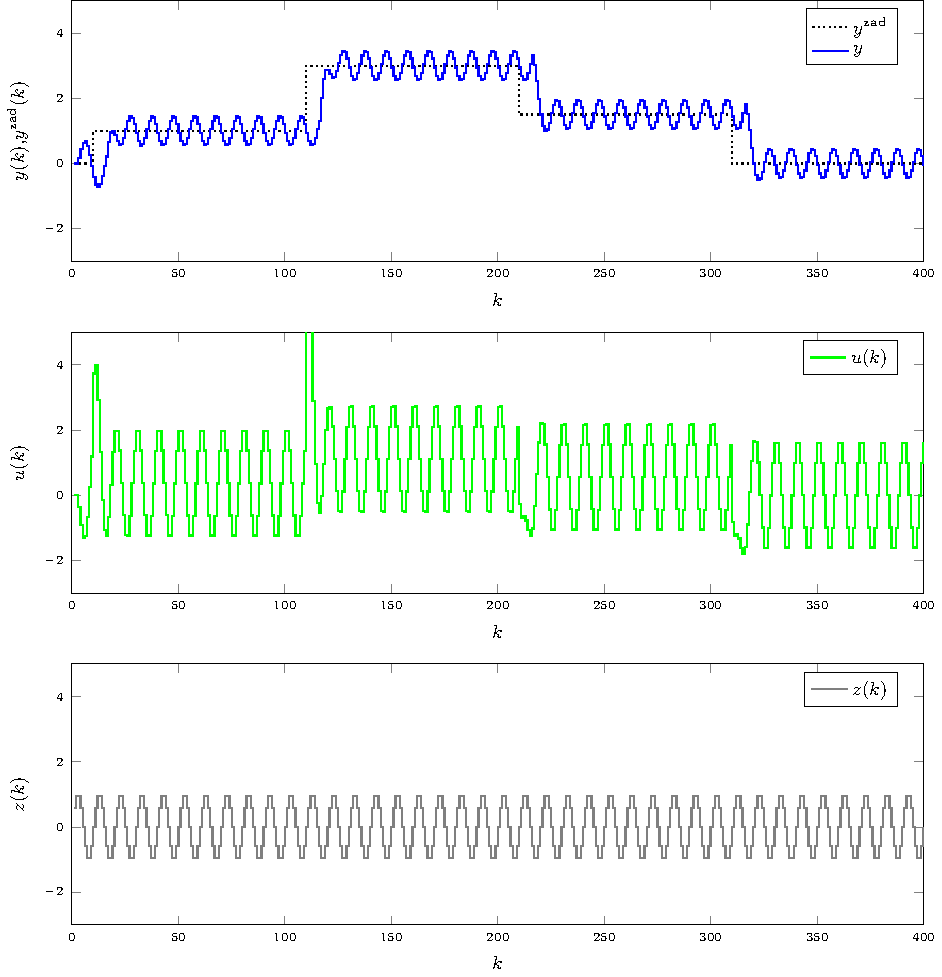
\includegraphics[width=\paperwidth]{data/exercise_6/Desired_output_plot_iter_06_ampl_1_freq_0.2_Dz_0_error_119.0913.pdf}}
\caption{amplitude=1, freq=0.2, Dz=0, error=119.0913}
\label{Desired_output_plot_iter_06_ampl_1_freq_0.2_Dz_0_error_119.0913}
\end{figure}
\end{center}
\begin{center}
\begin{figure}[H]
\makebox[\textwidth]{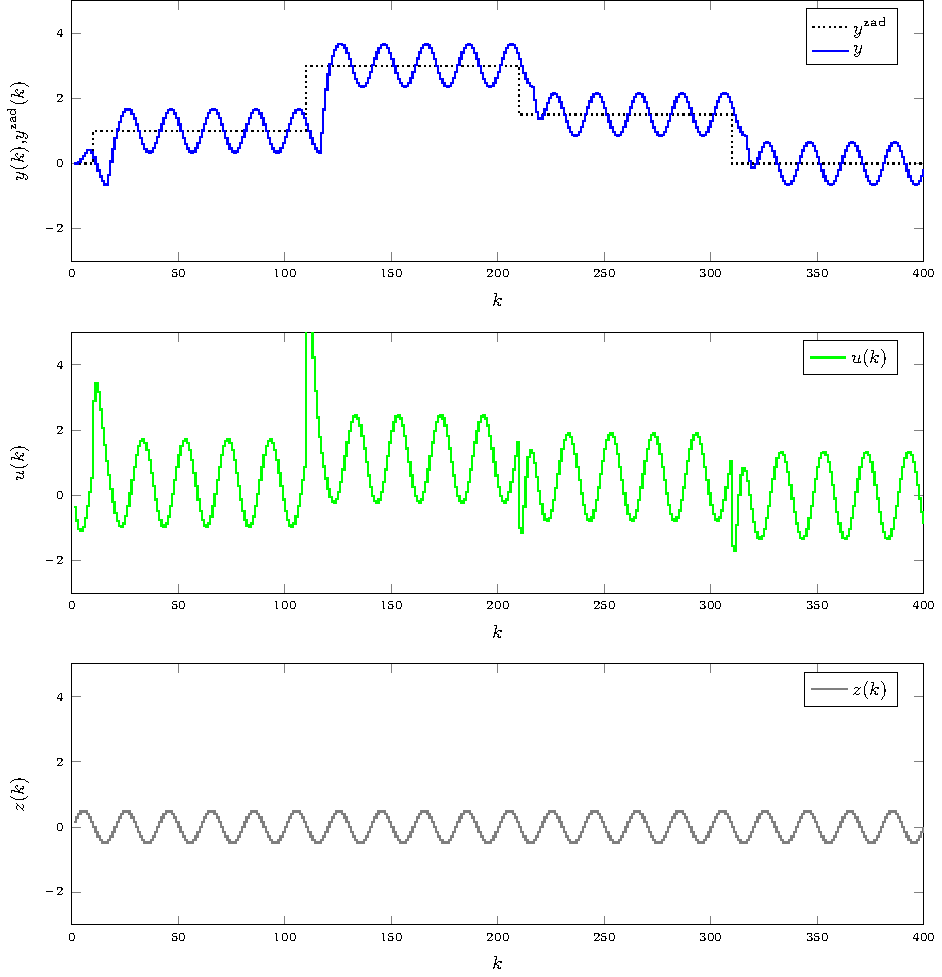
\includegraphics[width=\paperwidth]{data/exercise_6/Desired_output_plot_iter_07_ampl_0.5_freq_0.1_Dz_20_error_160.3299.pdf}}
\caption{amplitude=0.5, freq=0.1, Dz=20, error=160.3299}
\label{Desired_output_plot_iter_07_ampl_0.5_freq_0.1_Dz_20_error_160.3299}
\end{figure}
\end{center}
\begin{center}
\begin{figure}[H]
\makebox[\textwidth]{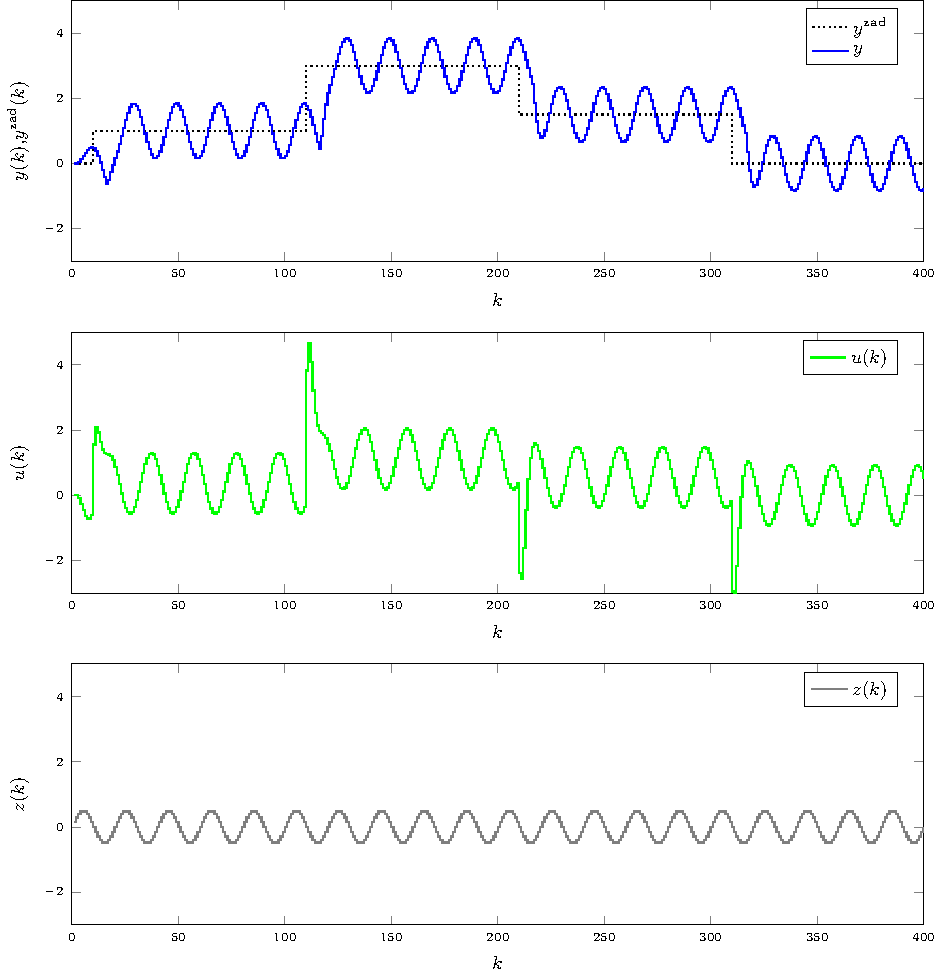
\includegraphics[width=\paperwidth]{data/exercise_6/Desired_output_plot_iter_08_ampl_0.5_freq_0.1_Dz_0_error_215.3014.pdf}}
\caption{amplitude=0.5, freq=0.1, Dz=0, error=215.3014}
\label{Desired_output_plot_iter_08_ampl_0.5_freq_0.1_Dz_0_error_215.3014}
\end{figure}
\end{center}

Jak mo�na zauwa�y�, r�nica w jako�ci regulacji na podstawie przebieg�w z i bez uwzgl�dniania sygna�u zak��caj�cego przez algorytm DMC przy obliczaniu sygna�u steruj�cego jest znacz�ca i tym wi�ksza, czym wy�sza jest amplituda sinusoidy zak��caj�cej.